\documentclass[12pt,spanish]{article}
\usepackage[utf8]{inputenc}
\usepackage{babel}
\usepackage{listings}
\usepackage{mathpazo}
\usepackage{enumitem}
\usepackage{courier}
\usepackage{textcomp}
\usepackage{xcolor}
\usepackage{parskip}
\usepackage{fullpage}

\newcommand{\onelinerule}{\rule[2.3ex]{0pt}{0pt}}
\newcommand{\twolinerule}{\rule[6.2ex]{0pt}{0pt}}
\newcommand{\respuesta}{\framebox[\textwidth]{\twolinerule}}
\newcommand{\nombre}{%
  \begin{tikzpicture}[xscale=.4,yscale=.7]
    \draw (0, 0) rectangle (22, 1);
  \end{tikzpicture}%
}
%\newcommand{\rol}   {\framebox[0.3\textwidth]{\onelinerule}}
\newcommand{\rol}{%
  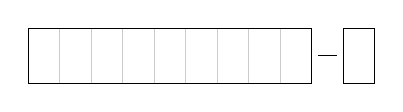
\begin{tikzpicture}[xscale=.4,yscale=.7]
    \draw[gray!40] ( 0, 0) grid      ( 9, 1);
    \draw          ( 0, 0) rectangle ( 9, 1);
    \draw          (10, 0) rectangle (11, 1);
    \draw (9 + .2, .5) -- (10 - .2, .5);
  \end{tikzpicture}%
}
\newcommand{\li}{\lstinline}
\newcommand{\pond}[1]{[{\small\textbf{#1\%}}]}

\lstdefinelanguage{py}{%
  classoffset=0,%
    morekeywords={%
      False,class,finally,is,return,None,continue,for,lambda,try,%
      True,def,from,nonlocal,while,and,del,global,not,with,print,%
      as,elif,if,or,yield,assert,else,import,pass,break,except,in,raise},%
    keywordstyle=\color{black!80}\bfseries,%
  classoffset=1,
    morekeywords={int,float,str,abs,len,raw_input,exit,range,min,max,%
      set,dict,tuple,list,bool,complex,round,sum,all,any,zip,map,filter,%
      sorted,reversed,dir,file,frozenset,open,%
      array,zeros,ones,arange,linspace,eye,diag,dot},
    keywordstyle=\color{black!50}\bfseries,%
  classoffset=0,%
  sensitive=true,%
  morecomment=[l]\#,%
  morestring=[b]',%
  morestring=[b]",%
  stringstyle=\em,%
}

\lstdefinelanguage{testcase}{%
  moredelim=[is][\bfseries]{`}{`},%
  backgroundcolor=\color{gray!20},%
}

\lstdefinelanguage{file}{%
  frame=single,%
  backgroundcolor=\color{white},%
}

\lstset{language=py}
\lstset{basicstyle=\ttfamily}
\lstset{columns=fixed}
\lstset{upquote=true}
\lstset{showstringspaces=false}
\lstset{rangeprefix=\#\ }
\lstset{includerangemarker=false}

\newlist{certamen}{enumerate}{1}
\setlist[certamen]{%
  label=\arabic*.,
  font=\LARGE\bfseries,%
  labelindent=-.5in,%
  leftmargin=0pt,%
  labelsep=1em%
}



\lstset{language=testcase,frame=single}

\begin{document}
  \thispagestyle{empty}
  \section*{Lunes 10 de septiembre}

  Escriba programas que permitan responder las siguientes preguntas:

  \begin{enumerate}
    \item ¿Es 991026973 un número primo?
      Si no lo es, ¿cuáles son sus divisores?
    \item ¿Cuántos números primos hay menores que diez mil?
    \item ¿Cuál es el tresmilésimo número primo?
    \item ¿Cuál es el producto de los diez primeros números primos
      que terminan en tres?
    \item ¿Cuáles son los treinta primeros números
      que son primos y palíndromos a la vez?
    \item ¿Cuál es el primer número primo cuyos dígitos suman 34?
      ¿Y 35?  ¿Y 36?
    \item ¿Cuántos pares de primos gemelos hay entre
      diez mil y cincuenta mil?
  \end{enumerate}

  Las siguientes definiciones le serán útiles.

  Un número es \emph{palíndromo} si se escribe igual de izquierda a derecha
  y de derecha a izquierda. Por ejemplo, 14285758241 y 11 son palíndromos.

  Dos números primos son \emph{gemelos} si su diferencia es dos.
  Por ejemplo, 17 y 19 son primos gemelos.
  Todos los pares de primos gemelos (excepto uno, ¿cuál?)
  son el antecesor y el sucesor de un múltiplo de seis.

\end{document}

